\chapter{文脈自由文法の世界}\label{ch03}
\index{ぶんみゃくじゆうぶんぽう@文脈自由文法}
\index{CFG}
\index{けいしきげんご@形式言語}

第2章では、JSONの構文解析器を記述することを通して、構文解析のやり方を学びました。構文解析器についても、PEG型の構文解析器および字句解析器を使った2通りを作ってみることで、構文解析器といってもいろいろな書き方があるのがわかってもらえたのではないかと思います。

この第3章では、現代の構文解析を語る上で必須である、文脈自由文法という概念について学ぶことにします。「文脈自由文法」というと、一見、堅くて難しそうな印象を持つ方も多いかもしれません。

しかし、実は皆さんはすでに文脈自由文法を使っているのです。Javaの\texttt{if}文やメソッド定義、JSONの入れ子構造など、プログラミングで日常的に扱っている「構造」はすべて文脈自由文法で表現されています。この章では、そんな身近な例から始めて、徐々に文脈自由文法の概念を理解していきましょう。

\section{身近な例から始める文脈自由文法}
\index{ぶんみゃくじゆうぶんぽう@文脈自由文法!例}
\index{いれここうぞう@入れ子構造}
\index{HTML}
\index{JSON}

まず、皆さんが普段書いているJavaコードを見てみましょう。以下はシンプルなif文です。

\begin{codescreen}{}
if (x > 0) {
    System.out.println("正の数です");
}
\end{codescreen}

このif文の構造を言葉で説明すると「\texttt{if}の後に条件式を括弧で囲み、その後に文のブロックがくる」となります。さらに、if文の中にif文を書くこともできます。

\begin{codescreen}{}
if (x > 0) {
    if (x > 100) {
        System.out.println("100より大きい");
    }
}
\end{codescreen}

この「入れ子にできる構造」こそが、文脈自由文法の本質なのです。

この入れ子構造は、プログラミング以外の場面でも頻繁に現れます。

\begin{itemize}
\item
  \textbf{\sffamily HTML}\textgt{の要素}：

\begin{codescreen}{}
<div>
    <p>段落の中に<strong>強調</strong>があり、
       さらに<a href="...">リンク</a>も含まれる</p>
</div>
\end{codescreen}
\item
  \textgt{数式の括弧}：

\begin{codescreen}{}
((2 + 3) × (4 - 1)) ÷ 5
\end{codescreen}
\item
  \textbf{日本語の引用}：

\begin{codescreen}{}
彼は「『明日は晴れる』と言った」らしい。
\end{codescreen}
\item
  \textbf{\sffamily JSON}\textgt{のオブジェクト}：

\begin{codescreen}{}
{
  "user": {
    "profile": {
      "name": "太郎"
    }
  }
}
\end{codescreen}
\end{itemize}

\enlargethispage{\baselineskip}これらの例に共通するのは、ある構造の中に同じような構造を含むことができ、その深さに制限がないという点です。このような構造を正確に記述し、解析するために文脈自由文法が必要になるのです。この問題は、次節で述べる「括弧の対応」という根本的な問題に帰着します。

\section{括弧の対応という根本問題}
\index{かっこのたいおう@括弧の対応}
\index{Dyck言語}
\index{いれここうぞう@入れ子構造}

形式言語で最も基本的で重要な構造の1つが「括弧の対応」です。大抵のプログラミング言語（JSONやYAMLのようなものも含む）は開き括弧と閉じ括弧に対応するルールを持っています。たとえ括弧そのものでなくても、\texttt{begin/end}や\texttt{\{\}}などが任意の深さだけ入れ子にできる場合は同じことです。

かなり原始的なプログラミング言語ですら、数式を入力できる機能があり、かつ数式の中で括弧を使うことができる以上、プログラミング言語の構文解析において括弧の対応は避けて通れない問題です。

さて、ここで括弧の対応とは何かを考えてみましょう。括弧の対応が取れているとは、\texttt{(}および\texttt{)}からなる文字列において、開き括弧と閉じ括弧が正しくペアになっていることを意味します。たとえば、以下は正しい括弧の対応です。

\begin{codescreen}{}
()          // 1組の括弧
(())        // 入れ子になった括弧
(()())      // 入れ子と並列の組み合わせ
()()()      // 並列に並んだ括弧
\end{codescreen}

一方、以下は正しくない例です。

\begin{codescreen}{}
)(          // 順序が逆
(()         // 閉じ括弧が不足
())         // 開き括弧が不足
\end{codescreen}

このような「\texttt{(}および\texttt{)}からなる文字列で、括弧の釣り合いが取れた文字列の並び」を表すものをDyck（ディック）言語と呼びます。「Dyck」は数学者の名前に由来しています。この、一見単純に見える問題が、構文解析において極めて重要な位置を占めているのです。

\section{BNFで括弧の構造を表現する}
\index{BNF}
\index{さいき@再帰}
\index{くうもじれつ@空文字列}
\index{いぷしろん@ε}

この括弧の対応をどのように文法として表現すればよいでしょうか？まずはすでに皆さんに学んでもらったBNFを使って考えてみましょう。

括弧の構造には以下の2つのパターンがあります。

\begin{enumerate}
\item
  空文字列（括弧なし）
\item
  \texttt{(} + 内側の括弧構造 + \texttt{)} + 続きの括弧構造
\end{enumerate}

これをBNFで書くと以下のようになります。

\begin{codescreen}{}
P = "(" P ")" P | "";
\end{codescreen}

\texttt{P}は「括弧のパターン」を表します。この定義は再帰的になっていることに注目してください。\texttt{P}の定義の中に\texttt{P}自身が現れています。これこそが、入れ子構造を表現する鍵なのです。

このBNFは上記の2つのパターンと直接対応しています。

\begin{itemize}
\item
  \texttt{"("\ P\ ")"\ P}：開き括弧、内側の構造、閉じ括弧、続きの構造（パターン1）
\item
  \texttt{""}：空文字列（パターン2）
\end{itemize}

\section{BNFから文脈自由文法へ}
\index{BNF}
\index{ぶんみゃくじゆうぶんぽう@文脈自由文法}
\index{せいせいきそく@生成規則}
\index{ひしゅうたんきごう@非終端記号}
\index{しゅうたんきごう@終端記号}
\index{かいしきごう@開始記号}

前節のBNFはすでに文脈自由文法の一種です。ただし、文脈自由文法の議論をする際には、より標準的な記法を使います。段階的に変換してみましょう。

\begin{itemize}
\item
  ステップ1: 選択を分離

まず、\texttt{\textbar{}}で区切られた選択肢を別々の規則に分けます。

\begin{codescreen}{}
P = "(" P ")" P;
P = "";
\end{codescreen}

同じ\texttt{P}が2つの規則で定義されていますが、これは「Pは2つのパターンのどちらかになる」という意味です。

\item
  ステップ2: 記号の変更

次に、記法を数学的な標準形に近づけます。

\begin{itemize}
\item
  \texttt{=} を \texttt{→}（生成規則を表す矢印）に変更
\item
  \texttt{""} を \texttt{ε}（イプシロン：空文字列を表す記号）に変更
\item
  文字を囲む引用符を削除
\end{itemize}

\begin{codescreen}{}
P → ( P ) P
P → ε
\end{codescreen}
\end{itemize}

これで文脈自由文法の標準的な記法になりました！

\subsection{用語の整理}

ここで重要な用語を整理しておきましょう。

\begin{itemize}
\item
  生成規則：\texttt{P\ →\ (\ P\ )\ P} のような矢印で結ばれた規則
\item
  非終端記号：\texttt{P}のような、さらに展開される記号（変数のようなもの）
\item
  終端記号：\texttt{(}や\texttt{)}のような、これ以上展開されない記号（実際の文字）
\item
  開始記号：文法の起点となる非終端記号（この例では\texttt{P}）
\end{itemize}

つまり、文脈自由文法とは以下のように表現できます。

\begin{itemize}
\item
  生成規則の集まり

  \begin{itemize}
  \item
    各生成規則は「非終端記号 → 記号の並び」の形
  \item
    記号の並びは終端記号と非終端記号の組み合わせ（空文字列εも可）
  \end{itemize}
\end{itemize}

これだけのシンプルなルールで、プログラミング言語の複雑な構文を表現できるのです。

\section{実例で理解する「言語」の概念}
\index{げんご@言語}
\index{けいしきげんご@形式言語}
\index{もじれつ@文字列}
\index{しゅうごう@集合}

前の節で定義したDyck言語の文法をもう一度見てみましょう。ここでは、文法の入口を明示するために、開始記号\texttt{D}とそれをPに置き換える規則\texttt{D → P}を先頭に加えています。

\begin{codescreen}{}
D → P
P → ( P ) P
P → ε
\end{codescreen}

この文法は括弧の対応を表すもの、というふうにぼかしてきました。実のところ、これまで出てきた文法はすべて「形式言語」を定義するものです。でも、ちょっと待ってください。「形式言語」って何でしょうか？

私たちが普段「プログラミング言語」と呼んでいるJavaやPythonと、この3行の規則で表される「括弧の言語」は、どう関係しているのでしょうか？実は、どちらも同じ「形式言語」という概念で理解できるのです。

\subsection{「形式言語」とは}

私たちが普段使う「言語」という言葉は、自然言語（日本語や英語など）を指すことが多いですが、理論の世界では「形式言語」という概念が重要です。形式言語とは、\textgt{文字列の集合}として定義される言語のことです。

ここで言う集合とは数学の集合のことです。形式言語の世界では文字列をひたすら集めていった、その集合が「言語」と呼ばれるのです。

単に「aabcaa」のような意味のない文字列の羅列に感じるかもしれませんが、重要なのは「どの文字列がその言語に属するか」という\textgt{規則}です。たとえば

\begin{itemize}
\item
  \textgt{パスワードの言語}：「8文字以上で、英数字と記号を含む文字列の集合」
\item
  \textgt{電話番号の言語}：「数字とハイフンからなる特定のパターンに従う文字列の集合」
\item
  \textgt{プログラミング言語}：「その言語の文法に従う正しいプログラムの集合」
\end{itemize}

つまり、形式言語は単なる文字列の寄せ集めではなく、明確な規則に基づいて「その言語に属する/属さない」が判定できる文字列の集合なのです。

さて、この観点から「Java言語」や「JavaScript言語」というとき、それは何を指しているのでしょうか？

\subsection{言語を「文字列の集合」として考える}

形式言語の立場からは、プログラミング言語を\textgt{その言語で書ける正しいプログラムすべての集合}として定義することができます。「正しいプログラム」といっても、構文解析ができるもの、型検査を通るもの、実行時にエラーが出ないものなど、いくつかの基準がありますが、ここでは「構文解析が通るプログラム」と考えます。

具体例で考えてみましょう。以下はすべて正しいJavaScriptプログラムです。

\begin{codescreen}{}
console.log("Hello, World!");
\end{codescreen}

\begin{codescreen}{}
console.log(3);
\end{codescreen}

\begin{codescreen}{}
console.log(3 + 5);
\end{codescreen}

これらを集めていくと、JavaScriptという言語（以後\texttt{JS}と表記）は次のような文字列の集合として表現できます。

\begin{codescreen}{}
JS = {
  "console.log(\"Hello, World!\");",
  "console.log(3);",
  "console.log(3 + 5);",
  "const x = 10;",
  "function add(a, b) { return a + b; }",
  ...（無限に続く）
}
\end{codescreen}

\enlargethispage{\baselineskip}JSで書ける正しいプログラムは無限にあるので、この集合は\textgt{無限集合}（正確には可算無限個の集合）になります。

\subsection{Dyck言語も集合として理解する}

同様に、Dyck言語（括弧の対応が取れた文字列）も集合として表現できます。

\begin{codescreen}{}
Dyck = {
  "()",
  "(())",
  "((()))",
  "(()())",
  "()()",
  "()()()",
  ...（無限に続く）
}
\end{codescreen}

Dyck言語も無限集合です。基本的に私たちが扱いたい言語＝集合は、ほとんどが無限集合です。なぜなら、基本的にはその言語のテキストがいくら長くなってもいいようにしたいからです。言語であらかじめ「長さの制限」を設けることは、実用的ではありません。

\subsection{集合として言語を扱うメリット}

言語を集合として扱うと、数学の集合論で使う記号が使えるようになります。これには実用的なメリットがあります。

まず、基本的な記号の意味を説明します。

\begin{itemize}
\item
  \texttt{∈}：「含まれる」を意味します（要素と集合の関係）
\item
  \texttt{∉}：「含まれない」を意味します（要素と集合の関係）
\item
  \texttt{⊂}：「部分集合」を意味します（集合と集合の関係）
\item
  \texttt{∩}：「共通部分」を意味します（両方の集合に含まれる要素）
\item
  \texttt{∪}：「和集合」を意味します（どちらかの集合に含まれる要素）（第6節で使用）
\end{itemize}

重要な違いとして、\texttt{∈}は要素（文字列）と集合（言語）の関係を表し、\texttt{⊂}は集合と集合の関係を表します。たとえば、以下のようになります。

\begin{codescreen}{}
"()" ∈ Dyck        // 「文字列"()"」が「言語Dyck」に含まれる
{""} ⊂ Dyck        // 「空文字列だけからなる集合」は「言語Dyck」の部分集合
\end{codescreen}

\begin{itemize}
\item
  例1：ある文字列が言語に含まれるかの判定

\begin{codescreen}{}
"()" ∈ Dyck         // "()"はDyck言語に含まれる
")(" ∉ Dyck         // ")("はDyck言語に含まれない
\end{codescreen}
\item
  例2：言語の後方互換性

Java 8がJava 5の後方互換であることを、集合の包含関係で表現できます。

\begin{codescreen}{}
Java5 ⊂ Java8     // Java 5で書けるプログラムはすべてJava 8でも書ける
\end{codescreen}
\item
  例3：言語の共通部分

たとえば、「JSでもTSでも有効なプログラム」は以下のように表現できます。

\begin{codescreen}{}
JS ∩ TS = {
  "console.log(123);",
  "const x = 5;",
  "function f() { return 1; }",
  ...
}
\end{codescreen}
\end{itemize}

このように、言語を集合として扱うことで、言語間の関係を明確に表現できるようになります。これは単なる理論ではなく、言語設計や互換性の議論において非常に役立ちます。

\section{文脈自由文法の数学的定義}
\index{ぶんみゃくじゆうぶんぽう@文脈自由文法!数学的定義}
\index{せいせいきそく@生成規則}
\index{ひしゅうたんきごう@非終端記号}
\index{しゅうたんきごう@終端記号}
\index{かいしきごう@開始記号}

ここまでふわっとした説明をしてきましたが、文脈自由文法の定義はもう少し厳密に行えます。本書では厳密な数学的扱いよりも実用的な理解を重視するため、あくまで厳密にはこう定義されるという話であって、この定義を直接使うことはありません。興味のない方は読み飛ばしても構いません。

文脈自由文法（Context-Free Grammar, CFG）は、形式的には4つ組
\(G = (V, \Sigma, P, S)\) として定義されます。

\begin{itemize}
\item
  \(V\)：非終端記号（Non-terminal symbols）の有限集合
\item
  \(\Sigma\)：終端記号（Terminal
  symbols）の有限集合（\(V \cap \Sigma = \emptyset\)）
\item
  \(P\)：生成規則（Production rules）の有限集合

  \begin{itemize}
  \item
    各規則は \(A \rightarrow \alpha\)
    の形（\(A \in V\)、\(\alpha \in (V \cup \Sigma)^*\)）
  \end{itemize}
\item
  \(S\)：開始記号（Start symbol）（\(S \in V\)）
\end{itemize}

たとえば、Dyck言語の文法は数学的には以下のように表せます。

\begin{itemize}
\item
  \(V = \{P\}\)
\item
  \(\Sigma = \{(, )\}\)
\item
  \(P = \{P \rightarrow (P)P, P \rightarrow \varepsilon\}\)
\item
  \(S = P\)
\end{itemize}

ここで \(\varepsilon\) は空文字列を表します。

文法 \(G\) が生成する言語 \(L(G)\) は、開始記号 \(S\)
から生成規則を繰り返し適用して導出できるすべての終端記号列の集合として定義されます。

\[L(G) = \{w \in \Sigma^* \mid S \Rightarrow^* w\}\]

ここで、\(\Rightarrow^*\) は「0回以上の導出ステップ」を表します。

もう少し噛み砕いて説明すると

\begin{enumerate}
\item
  開始記号 \(S\) から出発する
\item
  生成規則を適用して、非終端記号を置き換えていく
\item
  すべてが終端記号になったら、それが言語 \(L(G)\) の要素の1つ
\end{enumerate}

たとえば、Dyck言語の文法では以下のようになります。

\begin{itemize}
\item
  \(P \Rightarrow (P)P \Rightarrow ()P \Rightarrow ()\)
  という導出により、\texttt{()} が \(L(G)\) に含まれる
\item
  \(P \Rightarrow (P)P \Rightarrow ((P)P)P \Rightarrow (()P)P \Rightarrow (())P \Rightarrow (())\)
  により、\texttt{(())} も \(L(G)\) に含まれる
\item
  このようにして、すべての「正しく対応した括弧列」が \(L(G)\)
  の要素となる
\end{itemize}

この数学的定義を「きっちりと」理解することは、理論的には重要ですが、構文解析器の実装では、直感的な理解で問題ありません。BNFなどの記法は数学的定義と本質的に同じものを、より読みやすい形で表現しています。

\section{正規表現の限界と文脈自由言語}
\index{せいきひょうげん@正規表現}
\index{せいきげんご@正規言語}
\index{ぶんみゃくじゆうげんご@文脈自由言語}
\index{おーとまとん@オートマトン}
\index{ゆうげんおーとまとん@有限オートマトン}

ここまでで文脈自由文法の基本的な概念と言語を集合として扱う考え方を学びました。BNFと文脈自由文法の表現能力が実質的に等価であることはなんとなく理解できたかと思います。しかし、ここで1つ重大な疑問が浮かび上がります。それは、私たちにとってなじみ深い正規表現との関係です。正規表現も文脈自由文法と同じように言語＝文字列の集合を表現するためのツールですが、正規表現と文脈自由文法にはどのような違いがあるのでしょうか？

\subsection{身近な正規表現から考える}

皆さんは日常的に正規表現を使っているでしょう。ファイル検索、テキスト処理、入力値の検証など、さまざまな場面で活躍しています。

たとえば、Javaで電話番号の形式を簡易チェックするとき、以下のような正規表現を使うことがあります。

\begin{codescreen}{}
String phonePat = "\\d{3}-\\d{4}-\\d{4}";  // 例：090-1234-5678
if (phone.matches(phonePat)) {
    // 有効な電話番号
}
\end{codescreen}

あるいは、郵便番号の簡易チェックでは以下のような正規表現を使います。

\begin{codescreen}{}
String postalCodePat = "\\d{3}-\\d{4}";  // 例：123-4567
if (postalCode.matches(postalCodePat)) {
    // 有効な郵便番号
}
\end{codescreen}

正規表現は、特定のパターンにマッチする文字列を簡潔に表現できる強力なツールです。また、正規表現も無限集合を扱えます。上記の正規表現はあくまで有限個のパターンしか表せませんが、以下のパターンでは自然数を無限に表現できます。

\begin{codescreen}{}
String natPat = "0|[1-9][0-9]*";  // 0以上の自然数
if (number.matches(natPat)) {
    // 有効な自然数
}
\end{codescreen}

このとき、\texttt{natPat}は以下のような無限集合を表します。

\begin{codescreen}{}
{'0', '1', '2', '3', ...}
\end{codescreen}

注意してほしいのは、これはあくまで文字列としての自然数の集合であり、数値としての自然数ではないということです。正規表現は文字列のパターンを表現するためのツールであり、数値そのものを扱うわけではありません。

\subsection{正規表現でできないこと}

しかし、正規表現には決定的な限界があります。それは\textgt{括弧の対応が取れているかチェックできない}ということです。

試しに、すでにでてきたDyck言語を正規表現で判定することを考えてみましょう。

\begin{codescreen}{}
OK:  (), (()), (()(()))
NG:  )(, ((), ())
\end{codescreen}

どんなに工夫しても、任意の深さの括弧の対応を正規表現で表現することはできません。なぜでしょうか？次からは正規表現の基本的な仕組みとその限界について詳しく見ていきましょう。

\subsection{正規表現の構成要素を詳しく見る}

正規表現は、実は非常にシンプルな3つの基本演算から構成されています。現代の正規表現エンジンは多くの便利な記法を提供していますが、理論的にはすべて以下の1-3の基本演算に帰着できます（ただし、後方参照など「非正規表現」とでも呼ぶべき機能を除く）。

\subsubsection{連接（Concatenation）}

2つの正規表現を続けて書くことを\textgt{連接}と呼びます。

\begin{codescreen}{}
正規表現: ab
マッチする文字列: "ab"
マッチしない文字列: "a", "b", "ba", "abc"
\end{codescreen}

連接は最も基本的な演算で、「次に」という順序関係を表現します。

\subsubsection{選択（Alternation）}

\texttt{\textbar{}}記号を使って、複数の選択肢を表現します。

\begin{itemize}
\item
  正規表現: \texttt{a\textbar{}b}
\item
  マッチする文字列: \texttt{"a"}, \texttt{"b"}
\item
  マッチしない文字列: \texttt{"ab"}, \texttt{"c"}, \texttt{""}
\end{itemize}

より複雑な例：

\begin{itemize}
\item
  正規表現: \texttt{(ab\textbar{}cd)}
\item
  マッチする文字列: \texttt{"ab"}, \texttt{"cd"}
\item
  マッチしない文字列: \texttt{"ac"}, \texttt{"bd"}, \texttt{"abcd"}
\end{itemize}

\subsubsection{繰り返し（Kleene Star）}

\texttt{*}記号は、直前の要素を0回以上繰り返すことを意味します。この演算は数学者Stephen
Cole Kleene（スティーブン・クリーネ）にちなんで「Kleene
Star」と呼ばれます。

\begin{itemize}
\item
  正規表現: \texttt{a*}
\item
  マッチする文字列: \texttt{""}, \texttt{"a"}, \texttt{"aa"},
  \texttt{"aaa"}, \ldots{}
\item
  マッチしない文字列: \texttt{"b"}, \texttt{"ab"}
\end{itemize}

\subsubsection{派生的な演算子}

現代の正規表現では、より便利にするために多くの派生的な演算子が追加されています。

\begin{codescreen}{}
a+       1回以上の繰り返し（aa*と同等）
a?       0回または1回（a|εと同等）
a{n}     ちょうどn回の繰り返し
a{n,m}   n回以上m回以下の繰り返し
[a-z]    文字クラス（a|b|c|...|zと同等）
.        任意の1文字
\end{codescreen}

これらはすべて基本の3演算で表現できます。たとえば代表的な例をあげると以下のようになります。

\begin{itemize}
\item
  \texttt{a+} は \texttt{aa*}
\item
  \texttt{a?} は \texttt{a\textbar{}ε}（εは空文字列）
\item
  \texttt{{[}abc{]}} は \texttt{a\textbar{}b\textbar{}c}
\end{itemize}

\subsection{正規表現の裏側にある仕組み}

\enlargethispage{\baselineskip}皆さんは正規表現を使っているとき、その裏側でどのような処理が行われているか考えたことはありますか？実は、正規表現の限界を理解するには、その背後にある「オートマトン」という仕組みを知ることが役立ちます。「オートマトン」という名前は難しそうですが、要は「文字列を一文字ずつ読みながら状態を変えていく機械」のことです。

\subsubsection{オートマトンを自動販売機で考える}

オートマトンは「有限個の状態を持つ機械」です。難しく聞こえるかもしれませんが、自動販売機を例にするとわかりやすくなります。ここで、すべての商品は100円とし、投入可能な上限金額は300円とします。

\begin{itemize}
\item
  初期状態：お金が入っていない

  \begin{itemize}
  \item
    商品ボタンを押す → 初期状態のままで、お金が不足している旨を表示
  \item
    100円を投入 → 100円状態へ遷移
\end{itemize}
\item
  100円状態

  \begin{itemize}
  \item
    商品ボタンを押す → 商品を出して初期状態へ遷移
  \item
    商品ボタンを押さず100円投入 → 200円状態へ遷移
  \end{itemize}
\item
  200円状態

  \begin{itemize}
  \item
    商品ボタンを押す → 商品と、お釣り100円をだして初期状態へ遷移
  \item
    商品ボタンを押さず100円投入 → 300円状態へ遷移
  \end{itemize}
\item
  300円状態

  \begin{itemize}
  \item
    商品ボタンを押す → 商品と、お釣り200円をだして初期状態へ遷移
  \item
    商品ボタンを押さず100円投入 → 300円状態のまま、100円を返却
  \end{itemize}
\end{itemize}

図にすると以下のようになります。

\begin{center}
\begin{tikzpicture}[
  ->,>=stealth',
  node distance=3cm,
  initial text=start,
  every state/.style={thick, fill=gray!10},
  accepting/.style={double distance=2pt}
]

% 状態の定義
\node[state,initial] (q0) {初期状態};
\node[state] (q1) [right of=q0] {100円};
\node[state] (q2) [right of=q1] {200円};
\node[state] (q3) [right of=q2] {300円};

% 遷移の定義
% 100円投入による遷移
\path (q0) edge[bend left] node[above] {100円} (q1);
\path (q1) edge[bend left] node[above] {100円} (q2);
\path (q2) edge[bend left] node[above] {100円} (q3);
\path (q3) edge[loop above] node {100円/返} (q3);

% 商品ボタンによる遷移
\path (q0) edge[loop below] node {ボ/不} (q0);
\path (q1) edge[bend right=-30] node[below] {ボ/商} (q0);
\path (q2) edge[bend right=40] node[below] {ボ/（商，釣）} (q0);
\path (q3) edge[bend right=50] node[below] {ボ/（商，釣）} (q0);

\end{tikzpicture}
\end{center}

この図の見方を説明します。

\begin{itemize}
\item
  \textgt{ノード（状態）}：

  \begin{itemize}
  \item
    円で表現される各ノードが「状態」を表します
  \item
    「start」と書かれた矢印が指す「初期状態」から開始します
  \item
    各状態には現在の投入金額が記載されています
  \end{itemize}
\item
  \textgt{矢印（遷移）}：

  \begin{itemize}
  \item
    矢印は状態間の「遷移」を表します
  \item
    矢印上のラベルは「入力/出力」の形式です

    \begin{itemize}
    \item
      「100円」：100円硬貨を投入
    \item
      「ボ/商」：商品ボタンを押すと商品が出る
    \item
      「ボ/不」：商品ボタンを押すがお金が不足
    \item
      「ボ/（商，釣）」：商品ボタンを押すと商品とお釣りが出る
    \item
      「100円/返」：100円を投入するが満杯なので返却される
    \end{itemize}
  \end{itemize}
\item
  \textgt{動作の例}：

  \begin{enumerate}
  \item
    初期状態から100円を2回投入 → 200円状態へ
  \item
    200円状態で商品ボタンを押す → 商品とお釣りが出て初期状態へ戻る
  \end{enumerate}
\end{itemize}

この図は、自動販売機の「状態遷移」を完全に表現しています。どの状態からどの入力を受けたらどの状態に遷移するかが一目でわかります。

このように、オートマトンは「状態」と「入力」によって遷移を決定します。自動販売機では、状態はお金の投入状況で、入力はお金の投入や商品ボタンの押下です。

\subsubsection{簡単な例：ab*を認識するオートマトン}

このオートマトン（有限状態機械）を使うと正規表現で表現される言語を認識できます（正規表現で認識可能な言語はすべてオートマトンで表現可能と言い換えてもいいです）。ここでは、正規表現の例として
\texttt{ab*} を認識するオートマトンを考えてみましょう。

この正規表現は以下のような文字列にマッチします。

\begin{itemize}
\item
  \texttt{a}（bが0個）
\item
  \texttt{ab}（bが1個）
\item
  \texttt{abb}（bが2個）
\item
  \texttt{abbb}（bが3個）
\item
  \ldots{}
\end{itemize}

この正規表現を認識するオートマトンは以下のようになります。

\begin{center}
\begin{tikzpicture}[
  >=stealth',
  node distance=3cm,
  state/.style={circle, draw, minimum size=10mm},
  accept/.style={state, double}
]
  % 状態の定義
  \node[state] (s0) {0};
  \node[accept] (s1) [right of=s0] {1};

  % 遷移の定義
  \draw[->] (s0) -- node[above] {$a$} (s1);
  \draw[->] (s1) edge[loop above] node[above] {$b$} ();

  % 開始状態の矢印
  \draw[->] ([xshift=-1cm]s0.west) -- node[above] {開始} (s0);
\end{tikzpicture}
\end{center}

\begin{itemize}
\item
  状態0（開始状態）：最初の状態
\item
  状態1（受理状態）：この状態で入力が終わればマッチ成功
\item
  矢印：文字を読んだときの状態遷移
\end{itemize}

このオートマトンは以下のように動作します。

\begin{itemize}
\item
  入力\verb|"a"|：状態0→状態1（\textgt{受理}）
\item
  入力\verb|"ab"|：状態0→状態1→状態1（\textgt{受理}）
\item
  入力\verb|"abb"|：状態0→状態1→状態1→状態1（\textgt{受理}）
\item
  入力\verb|"b"|：状態0で\verb|"b"|を読めない（\textgt{非受理}）
\end{itemize}

\subsubsection{2種類のオートマトン}

オートマトンには大きく分けて2種類あります。難しい名前ですが、それぞれの特徴を簡単に説明します。

\begin{itemize}
\item
  \textbf{\sffamily NFA（Non-deterministic Finite
  Automaton}\textgt{、非決定性有限オートマトン）}

  \begin{itemize}
  \item
    「非決定性」とは、同じ文字を読んだときに複数の選択肢があることを指します
  \item
    文字を読まずに状態を移動できる（ε遷移）
  \item
    正規表現から比較的簡単に作れる
  \end{itemize}
\item
  \textbf{\sffamily DFA（Deterministic Finite Automaton}\textgt{、決定性有限オートマトン）}

  \begin{itemize}
  \item
    「決定性」とは、各状態で各文字に対して次の状態が一意に決まることを指します
  \item
    文字を読まずに移動することはできない
  \item
    実装が簡単で、実行速度が速い
  \end{itemize}
\end{itemize}

この2つのオートマトンは正規表現（正確には後で説明する正規言語）を認識するモデルであり、能力的には等価です。どちらも正規表現を認識できますが、実装の複雑さや速度に違いがあります。

ちなみに、これまで見てきたオートマトンはすべて状態遷移が一意に決まるDFAです。DFAは状態遷移が一意に決まるため、実装が非常にシンプルで高速です。

一方で、NFAはそのままでは実装が複雑で遅くなりますが、正規表現からの変換が容易であるという利点があります。

\subsection{なぜ正規表現では括弧の対応が扱えないのか}

ここまで、正規表現がオートマトンという仕組みで動作することを学びました。では、なぜオートマトン（正規表現）では括弧の対応がチェックできないのでしょうか？その理由を理解するために、簡単な例から考えてみましょう。

括弧の対応を確認するには、以下のような処理が必要です。

\begin{itemize}
\item
  \texttt{(}を読んだら、「今までに読んだ開き括弧の数」を1増やす
\item
  \texttt{)}を読んだら、「対応する開き括弧があるか」確認して、1減らす
\item
  最後に、カウントが0であることを確認する
\end{itemize}

ここで問題になるのは、括弧は何重にでもネスト（入れ子）できるということです。たとえば以下のようなケースを扱える必要があります。

\begin{itemize}
\item
  \texttt{(())}：2重
\item
  \texttt{((()))}：3重
\item
  \texttt{(((())))}：4重
\item
  \ldots 無限に続く
\end{itemize}

\subsubsection{オートマトンの限界：有限の状態しか持てない}

オートマトンは「有限個の状態」しか持てません。仮に10個の状態を持つオートマトンを作ったとしても、11重にネストした括弧は扱えません。どんなに状態数を増やしても、それを超える深さのネストが存在します。

これを具体的に理解するために、簡単なオートマトンで考えてみましょう。仮に「最大3つまでの開き括弧を数える」オートマトンを作ると次のようになります。

\begin{center}
\begin{tikzpicture}[
  >=stealth',
  node distance=2.5cm,
  state/.style={circle, draw, minimum size=10mm},
  accept/.style={state, double},
  every edge/.style={draw, ->, >=stealth'}
]
  % 状態の定義
  \node[accept] (s0) {0};
  \node[state] (s1) [right of=s0] {1};
  \node[state] (s2) [right of=s1] {2};
  \node[state] (s3) [right of=s2] {3};
  \node[state] (err) [below of=s1] {エラー};

  % 開き括弧による遷移
  \draw (s0) edge[bend left] node[above] {(} (s1);
  \draw (s1) edge[bend left] node[above] {(} (s2);
  \draw (s2) edge[bend left] node[above] {(} (s3);
  \draw (s3) edge[bend right=-40] node[right] {(} (err);

  % 閉じ括弧による遷移
  \draw (s1) edge[bend left] node[below] {)} (s0);
  \draw (s2) edge[bend left] node[below] {)} (s1);
  \draw (s3) edge[bend left] node[below] {)} (s2);
  \draw (s0) edge node[left] {)} (err);

  % 開始状態の矢印
  \draw[->] ([xshift=-1cm]s0.west) -- (s0);
\end{tikzpicture}
\end{center}

このオートマトンは3つまでの開き括弧なら正しく数えられますが、4つ目の開き括弧がくるとエラー状態に遷移してしまいます。状態数を100個に増やしても、101個の開き括弧には対応できません。

\subsection{実用上の意味}

この違いは実用上極めて重要です。以下のような違いがあるからです。

\begin{itemize}
\item
  正規表現で十分な例：

  \begin{itemize}
  \item
    URLの検証
  \item
    電話番号のフォーマットチェック
  \item
    単純なトークンの切り出し
  \item
    メールアドレスの簡単な検証
  \end{itemize}
\item
  文脈自由文法が必要な例：

  \begin{itemize}
  \item
    プログラミング言語の構文解析
  \item
    JSONやYAML、XMLのパース
  \item
    数式の評価（括弧を含む）
  \item
    メールアドレスの完全な検証
  \end{itemize}
\end{itemize}

\subsection{メールアドレスと正規表現の注意点}

メールアドレスの検証は簡単だと思われがちですが、完全な仕様（RFC
5322）は非常に複雑で、厳密にはコメントの入れ子などを許可するため、正規表現では表現しきれません。たとえば、以下のような入れ子構造をもったメールアドレスも仕様上は有効です。

\begin{codescreen}{}
john.doe@(comment)example.com
john.doe@(comment1(comment2))example.com
\end{codescreen}

実用上はaddr-spec（\texttt{local-part@domain}の形式）の簡略化されたパターンを正規表現で検証するのが一般的ですが、完全な仕様準拠が必要な場合は、専用のパーサーを使用するべきです。

メールアドレスの検証ですら、完全な仕様準拠を目指すなら文脈自由文法の理解が必要になるのです。

\subsection{なぜ「文脈自由」なのか？}

ここまで文脈自由文法について学んできましたが、なぜ「文脈自由」という名前なのでしょうか？これは、対となる概念である「文脈依存文法」と比較すると理解しやすくなります。

\bigskip
\noindent\textgt{文脈自由の例}：

\begin{codescreen}{}
A → abc
\end{codescreen}

この規則では、Aはどこに現れても常に\texttt{abc}に置き換えられます。周りの文脈（前後の文字）に関係なく適用できるので「文脈自由」です。自由というと一見「好きにできる」という印象を受けますが、ここの「自由」は、たとえば、アルコールフリー＝アルコールが含まれない、という意味での「自由」です。形式言語を扱う研究者の中にはContext-free Grammarを「文脈自由文法」と訳したのは誤解を招きやすいので、あまりよくなかったのではないか、という人もいます。

\bigskip
\noindent\textgt{文脈依存の例}：

\begin{codescreen}{}
xAy → xabcy
\end{codescreen}

この規則では、Aが\texttt{x}と\texttt{y}に挟まれている時だけ\texttt{abc}に置き換えられます。文脈（周りの文字）に依存しているので「文脈依存」です。

プログラミング言語の構文のほとんどは文脈自由文法で表現できます。たとえば、\texttt{if}文の中に\texttt{if}文を書けるのは、外側の文脈に関係なく同じ規則が適用できるからです。一方、「変数は使用前に宣言されていなければならない」のような規則は文脈依存であり、構文解析とは別の段階（意味解析）で扱われます。

以下で形式言語の階層をまとめてみます。

\begin{itemize}
\item
  正規言語（RL: Regular Language）：

  \begin{itemize}
  \item
    正規表現で表現できる\textgt{言語の集合}
  \item
    例：電話番号、識別子、単純なパターン
  \end{itemize}
\item
  文脈自由言語（CFL: Context-Free Language）：

  \begin{itemize}
  \item
    文脈自由文法で表現できる\textgt{言語の集合}
  \item
    例：プログラミング言語の構文、JSON、XML
  \item
    正規言語をすべて含む（RL ⊂ CFL）
  \end{itemize}
\item
  文脈依存言語（CSL: Context-Sensitive Language）:

  \begin{itemize}
  \item
    文脈依存文法で表現できる\textgt{言語の集合}
  \item
    例：$a^nb^nc^n$ （n個のa、b、cがこの順で並ぶ集合）
  \item
    文脈自由言語をすべて含む（CFL ⊂ CSL）
  \end{itemize}
\item
  帰納的可算言語（RE: Recursively Enumerable Language）:

  \begin{itemize}
  \item
    （汎用）コンピュータが出力できるすべての記号列の集合
  \item
    JavaやPythonなどのプログラミング言語の計算能力はこのレベル
  \item
    文脈依存言語をすべて含む（CSL ⊂ RE）
  \end{itemize}
\end{itemize}

階層を図にすると次のようになります。この図は言語の表現力の階層を表しており、内側の言語クラスは外側の言語クラスに完全に含まれます（包含関係）。

\begin{center}
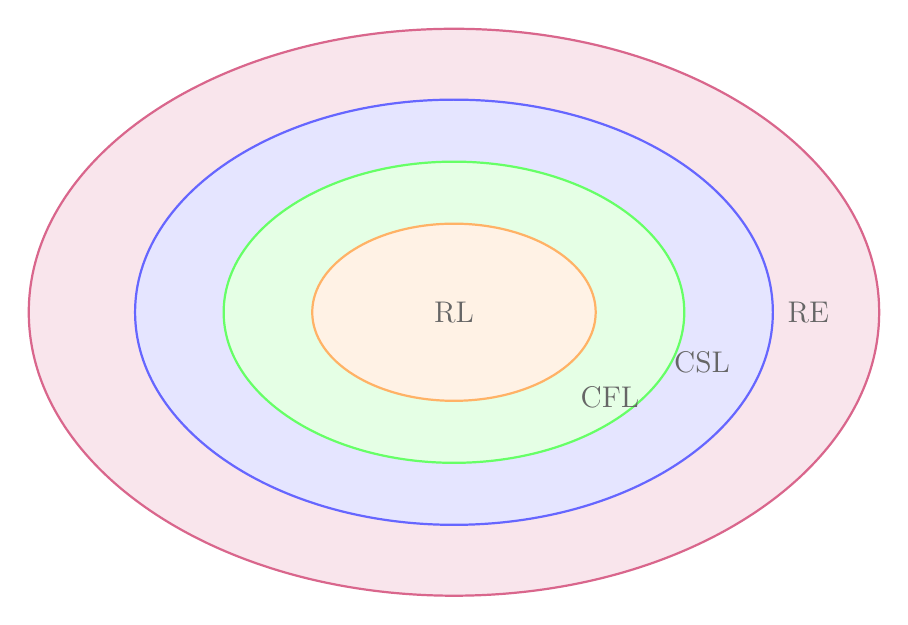
\begin{tikzpicture}[scale=0.9, transform shape]
  % 最外側の楕円 (RE)
  \draw[fill=purple!10,draw=purple!60,thick] (0,0) ellipse (6cm and 4cm);
  \node at (5.0,0) {\textcolor{black!60}{\large RE}};

  % 文脈依存言語 (CSL)
  \draw[fill=blue!10,draw=blue!60,thick] (0,0) ellipse (4.5cm and 3cm);
  \node at (3.5,-0.7) {\textcolor{black!60}{\large CSL}};

  % 文脈自由言語 (CFL)
  \draw[fill=green!10,draw=green!60,thick] (0,0) ellipse (3.25cm and 2.125cm);
  \node at (2.2,-1.2) {\textcolor{black!60}{\large CFL}};

  % 正規言語 (RL)
  \draw[fill=orange!10,draw=orange!60,thick] (0,0) ellipse (2cm and 1.25cm);
  \node at (0,0) {\textcolor{black!60}{\large RL}};
\end{tikzpicture}
\end{center}

プログラミング言語の\textgt{構文}は文脈自由文法で記述できますが、プログラミング言語自体の\textgt{計算能力}はチューリング完全（最上位）です。この違いを理解することが重要です。

\section{文法から文字列を作る：導出の仕組み}
\index{どうしゅつ@導出}
\index{さいさどうしゅつ@最左導出}
\index{さいうどうしゅつ@最右導出}
\index{かいせきぎ@解析木}

文脈自由文法は「生成規則」の集まりでした。では、この「生成」とは何でしょうか？

Dyck言語の文法をもう一度見てみましょう。

\begin{codescreen}{}
D → P
P → ( P ) P
P → ε
\end{codescreen}

これらの規則は「置き換えルール」として読めます。

\begin{itemize}
\item
  \texttt{D\ →\ P}：「Dを見たらPに置き換えてよい」
\item
  \texttt{P\ →\ (\ P\ )\ P}：「Pを見たら( P ) Pに置き換えてよい」
\item
  \texttt{P\ →\ ε}：「Pを見たら空文字列に置き換えてよい」
\end{itemize}

\subsection{実際に文字列を生成してみる}

\texttt{()}という文字列を生成する過程を追ってみましょう。

\begin{codescreen}{}
D               // 開始記号から始める
→ P            // D → P を適用
→ ( P ) P      // P → ( P ) P を適用
→ ( ε ) P     // 最初のPに P → ε を適用
→ ( ) P        // εは空文字列なので消える
→ ( ) ε       // 2番目のPに P → ε を適用  
→ ( )          // εは空文字列なので消える
\end{codescreen}

このように、規則を順番に適用して文字列を作ることを\textgt{導出}と呼びます。生成すると言い換えてもよいでしょう。

\subsection{複数の導出方法}

同じ文字列を導出する方法は複数あります。簡単な文法で考えてみましょう。

\begin{codescreen}{}
S → AB
A → a
B → b
\end{codescreen}

この文法から\texttt{ab}を導出するとき、どちらから先に展開するかで2通りの方法があります。

\begin{itemize}
\item
  方法1（左から展開）：
\begin{codescreen}{}
S → AB → aB → ab
\end{codescreen}
\item
  方法2（右から展開）：
\begin{codescreen}{}
S → AB → Ab → ab
\end{codescreen}
\end{itemize}

\subsection{最左導出と最右導出}

このように好きな順番で非終端記号を展開できるのですが、導出の過程を統一するために2つの標準的な方法が定義されています。

\begin{itemize}
\item
  \textgt{最左導出}：常に一番左の非終端記号を展開
\item
  \textgt{最右導出}：常に一番右の非終端記号を展開
\end{itemize}

簡単な例で見てみましょう。以下の文法は「1個以上のa」の後に「1個以上のb」が続く文字列を表します。

\begin{codescreen}{}
S → AB
A → aA | a
B → bB | b
\end{codescreen}

\texttt{aabb}を導出する場合

\begin{itemize}
\item
  \textgt{最左導出：}
\begin{codescreen}{}
S  
→ AB      (S → AB)
→ aAB     (A → aA)  
→ aaB     (A → a)
→ aabB    (B → bB)
→ aabb    (B → b)
\end{codescreen}

\item
  \textgt{最右導出：}
\begin{codescreen}{}
S
→ AB      (S → AB)
→ AbB     (B → bB)
→ Abb     (B → b)  
→ aAbb    (A → aA)
→ aabb    (A → a)
\end{codescreen}
\end{itemize}

\subsection{解析木との関係}

どちらの導出方法でも、最終的に同じ\textgt{解析木}が得られます。

\begin{center}
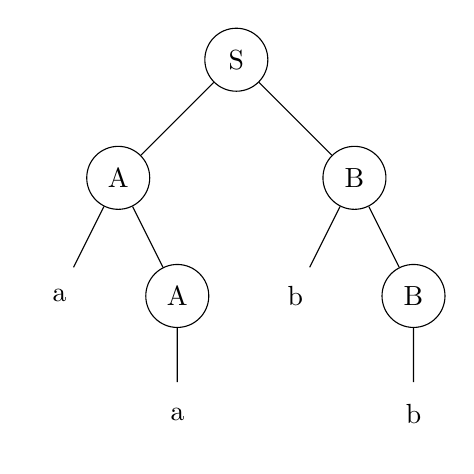
\begin{tikzpicture}[
  level distance=1.5cm,
  level 1/.style={sibling distance=3cm},
  level 2/.style={sibling distance=1.5cm},
  every node/.style={circle, draw, minimum size=8mm}
]
  \node {S}
    child {node {A}
      child {node[circle, draw=none] {a}}
      child {node {A}
        child {node[circle, draw=none] {a}}
      }
    }
    child {node {B}
      child {node[circle, draw=none] {b}}
      child {node {B}
        child {node[circle, draw=none] {b}}
      }
    };
\end{tikzpicture}
\end{center}

最左導出は木を左から右へ構築し、最右導出は右から左へ構築するイメージです。ここで得られた解析木は具体的な文字列の情報を含んでおり、抽象構文木と対比する形で具象構文木と呼ばれることもあります。

\subsection{なぜ2つの導出方法が重要か}

これらの導出方法は、構文解析の2つのアプローチと関連があります。

\begin{itemize}
\item
  \textgt{下向き構文解析}（トップダウン）：文法の開始記号から始めて、入力に合うよう規則を適用していく
\item
  \textgt{上向き構文解析}（ボトムアップ）：入力から始めて、段階的に規則を適用して開始記号まで到達する
\end{itemize}

第2章で作ったJSONパーサーは下向き構文解析の一種でした。ただし、導出と構文解析の対応関係は複雑で、最左導出と下向き構文解析が常に一対一で対応するわけではありません。次章では、これらの手法の実際の動作についてより詳しく学んでいきます。

\section{まとめ}

この章では、文脈自由文法について学びました。最初は難しく感じたかもしれませんが、実は私たちが普段書いているプログラムと深く関わっている概念です。この章で学んだことを整理します。

\begin{enumerate}
\item
  文脈自由文法の基礎

  \begin{itemize}
  \item
    Javaのif文やJSONの構造など、プログラミングの「入れ子構造」は文脈自由文法で表現される
  \item
    BNFから文脈自由文法への変換は記法の違いに過ぎない
  \item
    生成規則、非終端記号、終端記号という基本要素で構成される
  \end{itemize}
\item
  言語を集合として理解する

  \begin{itemize}
  \item
    プログラミング言語は「正しいプログラムの集合」として定義できる
  \item
    集合論の記法を使って言語間の関係を厳密に議論できる
  \item
    後方互換性なども集合の包含関係として表現可能
  \end{itemize}
\item
  正規表現とオートマトン

  \begin{itemize}
  \item
    正規表現は正規言語を表現するための強力なツール
  \item
    NFA（非決定性有限オートマトン）とDFA（決定性有限オートマトン）の違い
  \item
    正規表現は有限の状態しか持てないため、括弧の対応などの複雑な構造を扱えない
  \end{itemize}
\item
  言語の階層

  \begin{itemize}
  \item
    正規表現（正規言語）\textless{}
    文脈自由文法（文脈自由言語）\textless{} \ldots{} 帰納的可算言語
  \item
    プログラミング言語の構文解析には文脈自由文法が必要
  \end{itemize}
\item
  導出の仕組み

  \begin{itemize}
  \item
    生成規則を適用して文字列を生成する過程が導出
  \item
    最左導出と最右導出という2つの標準的な方法がある
  \item
    これらは下向き/上向き構文解析に対応する
  \end{itemize}
\end{enumerate}

文脈自由文法の理解は、以下の場面で役立ちます。

\begin{itemize}
\item
  \textgt{構文解析器の実装}：第4章以降で学ぶさまざまな構文解析アルゴリズムの基礎
\item
  \textgt{言語設計}：新しいDSLやプログラミング言語を設計する際の指針
\item
  \textgt{エラーメッセージの理解}：コンパイラのエラーメッセージがなぜそう言っているかの理解
\item
  \textgt{ツールの選択}：正規表現で十分か、パーサーが必要かの判断
\end{itemize}

次章ではこの文脈自由文法を元に、実際の構文解析アルゴリズムについて詳しく見ていきます。
